\documentclass[a4paper,fleqn]{cas-dc}

\usepackage[authoryear,longnamesfirst]{natbib}
\usepackage{amssymb}
\usepackage{graphicx}
\usepackage{url}
\usepackage{placeins}
\usepackage{booktabs}

\begin{document}
\let\WriteBookmarks\relax
\def\floatpagepagefraction{1}
\def\textpagefraction{.001}

\shorttitle{Reliability and Security of LLM-Generated Kubernetes Configurations}
\shortauthors{N. Ali and T. Hussain}

\title[mode = title]{Reliability and Security Analysis of LLM-Generated Kubernetes Configurations: A Project-Matched Comparison of Human-Written and Multi-LLM Manifests}

\author[1]{Nabeed Ali}
\author[1]{Talha Hussain}

\affiliation[1]{organization={Department of Software Engineering, NED University of Engineering and Technology},
            city={Karachi},
            country={Pakistan}}

\begin{abstract}
Large language models (LLMs) are increasingly used to write Kubernetes configurations, yet misconfigured manifests can expose clusters to privilege escalation, resource exhaustion and service outages. Prior studies of LLM-generated Kubernetes manifests rely on a single 2023 model, uncontrolled prompts, one static analysis tool and no execution, and they do not compare against human-written configurations of the same applications. This study will empirically evaluate the reliability and security of Kubernetes configurations generated by five current proprietary and open-weight LLMs for a set of real open-source applications, using the manifests that the maintainers ship as a reference point. Each model receives only the project's own documentation, with Kubernetes-specific content redacted, under a neutral and a production-oriented prompt, and all generated and human-written configurations will pass through a six-dimension benchmark covering correctness, security, static reliability, requirement satisfaction, real deployment and fault-injection recovery. This preprint presents the motivation, related work and study design; experimental results are not yet available.
\end{abstract}

\begin{keywords}
Kubernetes \sep Large Language Models \sep Infrastructure as Code \sep Security Misconfiguration \sep Reliability \sep Empirical Study
\end{keywords}

\maketitle

\section{Introduction}\label{sec:intro}

Kubernetes has become the de-facto platform for orchestrating containerised applications, and organisations increasingly rely on it to deploy, scale and operate production software \citep{rahman2023k8smisconfig,shamim2020xicommandments}. The behaviour of a Kubernetes workload is not defined in application code but in declarative configuration files, known as \emph{manifests}, which specify, among other things, how many replicas run, how the health of containers is probed, how much CPU and memory each container may consume, which privileges it holds and how it is exposed on the network. Because these settings directly determine the security posture and the availability of the running system, errors in manifests have operational and security consequences. Configuration mistakes can grant containers root or host-level privileges, leak secrets, allow resource exhaustion, or leave a service unavailable when a pod fails \citep{rahman2023k8smisconfig,zhang2026k8sconfigdefects,nsacisa2022k8shardening}. Writing correct, secure and reliable manifests is therefore an important but error-prone engineering task.

Empirical studies show that human-written manifests frequently contain such problems. Rahman et al.\ identified 1,051 security misconfigurations across 2,039 manifests mined from 92 open-source repositories and grouped them into 11 categories, such as absent resource limits, absent security contexts and privileged containers \citep{rahman2023k8smisconfig}. Zhang et al.\ later catalogued 15 categories of Kubernetes configuration defects, including probing, resource and scheduling defects, and found that eight widely used static analysis tools detect only 8 of these 15 categories \citep{zhang2026k8sconfigdefects}. In parallel, large language models (LLMs) such as ChatGPT, Claude and Gemini, together with open-weight models such as Llama, Qwen and DeepSeek, have become everyday assistants for software and infrastructure engineering. They are now routinely asked to produce Kubernetes manifests directly from natural-language descriptions \citep{zhang2024genaismells}. Research on general-purpose code has repeatedly shown that LLM assistants reproduce insecure patterns: around 40\% of programs generated by GitHub Copilot in security-relevant scenarios were vulnerable \citep{pearce2022asleep}, and around half of the functionally correct backends generated by state-of-the-art models were exploitable \citep{vero2025baxbench}. For infrastructure-as-code, syntactic validity and deployability have been found to be largely independent of security compliance \citep{santosvargas2026secureterraform,zhang2026iacgen}.

Despite this growing reliance on LLMs, the quality of LLM-generated Kubernetes configurations is still poorly understood. The first study on the topic analysed 98 ChatGPT-generated manifests collected from developer conversations and found that 35.8\% contained unset CPU and memory requirements \citep{zhang2024genaismells}. However, it relied on uncontrolled prompts, a single model from 2023, a single static analysis tool and no human baseline. A subsequent comparison with human-written manifests \citep{jcomsec2026aivshumank8s} re-used those 2023 ChatGPT measurements against an unrelated human corpus and, as its authors state, did not generate new manifests with newer models, relied on a single tool, and did not execute any manifest in a cluster. Benchmarks for LLM-generated cloud configuration, such as CloudEval-YAML \citep{xu2024cloudevalyaml} and FDE-Bench \citep{ding2026fdebench}, evaluate curated tasks rather than real projects and do not compare against the manifests that developers actually ship. Other Kubernetes-specific LLM research uses models to \emph{detect}, \emph{repair} or \emph{harden} existing manifests rather than to author them \citep{malul2024genkubesec,ye2025llmsecconfig,sgancohen2025kubeguard}. Consequently, there is no evidence on (i) how configurations produced by current LLMs compare with human-written configurations \emph{for the same applications}, (ii) how different LLMs compare with each other under identical requirements, and (iii) whether these configurations actually deploy and recover from failures in a real cluster, which is where their reliability ultimately matters.

The main objective of this study is to empirically evaluate the reliability and security of Kubernetes configurations generated by LLMs, using the configurations that the same real-world projects actually ship as a reference point. Specifically, the study addresses the following research questions:
\begin{itemize}
    \item \textbf{RQ1:} How do LLM-generated Kubernetes configurations compare with the human-written configurations shipped by the same projects in correctness, security, reliability, requirement satisfaction and runtime behaviour?
    \item \textbf{RQ2:} Which errors and misconfigurations occur most frequently in LLM-generated configurations?
    \item \textbf{RQ3:} How do different LLMs differ in the type and frequency of the problems they introduce, and how consistent is each model across repeated generations?
    \item \textbf{RQ4:} How reliably do LLM-generated configurations deploy and recover from failures in a real Kubernetes cluster compared with human-written configurations, and do static analysis findings predict these runtime outcomes?
    \item \textbf{RQ5:} Does explicitly requesting production-ready output change the security and reliability of LLM-generated configurations?
\end{itemize}

To answer these questions, this study selects seven non-trivial open-source applications whose maintainers ship Kubernetes manifests, ranging from stateful database-backed applications and multi-service microservice systems to a cluster add-on. For each application, every LLM receives the same \emph{docs bundle}: the project's own README, Dockerfile and Docker Compose file, copied verbatim from the repository at a pinned commit, with Kubernetes-specific passages (embedded manifests and deployment instructions) redacted. No specification is authored by the research team; the model sees exactly what the project's maintainers wrote, so the comparison cannot be confounded by a researcher's or an LLM's own wording. The same bundle is given to five LLMs: three proprietary models (OpenAI GPT, Anthropic Claude and Google Gemini) and two open-weight models (Qwen and DeepSeek). Because the human developers did not necessarily aim for production-grade manifests, two prompt variants are used. A neutral prompt asks only for manifests that deploy the application and is used for the comparison with the human-written configurations, which are additionally classified as production- or demonstration-oriented. A second prompt explicitly requests production-ready manifests and is used to measure the effect of the request itself. Each model generates three independent samples per project and prompt variant, and the resulting LLM-generated configurations are evaluated together with the human-written configurations shipped by the same projects. All configurations pass through the same automated evaluation pipeline, organised as a six-dimension benchmark. The dimensions are (D1) correctness, using kubeconform and server-side validation; (D2) security, using Kubescape, Trivy and the Kubernetes Pod Security Standards; (D3) static reliability, using kube-score, Polaris, KubeLinter and a reliability-controls checklist; (D4) requirement satisfaction against a fact sheet of the application's documented requirements; (D5) actual deployment on a disposable Kubernetes cluster with a functional smoke test; and (D6) resilience, measured through pod-deletion and container-crash fault-injection experiments that record recovery time and service availability. Results are compared across sources using non-parametric statistical tests and effect sizes.

The main contributions of this paper are as follows:
\begin{itemize}
    \item A \emph{project-matched} empirical comparison of human-written and LLM-generated Kubernetes configurations, in which every LLM receives the same real application's own documentation, with no researcher- or model-authored specification in between.
    \item A systematic comparison of five current proprietary and open-weight LLMs on Kubernetes configuration generation, including their consistency across repeated samples and their sensitivity to an explicit request for production-ready output.
    \item A six-dimension evaluation benchmark that links static correctness, security and reliability analysis to requirement satisfaction, real deployment and fault-injection-based recovery, making it possible to test whether static findings predict runtime behaviour.
    \item A replication package containing the docs bundles, prompts, raw model outputs, generated manifests, tool outputs and analysis scripts.
\end{itemize}

The rest of this paper is organised as follows. Section~\ref{sec:literature} reviews related work on Kubernetes misconfigurations, the security of LLM-generated code, LLM-based generation of infrastructure configurations, and LLM-based analysis and repair of Kubernetes manifests, and identifies the research gap. Section~3 describes the dataset, the generation procedure and the evaluation benchmark. Section~4 presents the experimental results for each research question. Section~5 discusses the findings and their implications for practitioners, and Section~6 discusses threats to validity. Finally, Section~7 concludes the paper and outlines directions for future research.

\section{Related Work}\label{sec:literature}

This section reviews six lines of prior work. Section~\ref{sec:comparative} compares the closest studies with ours and states the research gap.

\subsection{Misconfigurations in human-written Kubernetes configurations}\label{sec:lit-human}

Rahman et al.\ identified seven security smells in Puppet scripts, such as hard-coded secrets \citep{rahman2019sevensins}. For Kubernetes, Shamim et al.\ organised practitioner knowledge into eleven recommended security practices \citep{shamim2020xicommandments}. The most complete study of Kubernetes security misconfigurations analysed 2,039 manifests from 92 open-source repositories. Its 11 categories, such as absent resource limits and privilege escalation, affected 13.9\% of the analysed objects \citep{rahman2023k8smisconfig}. Beyond security, \citet{zhang2026k8sconfigdefects} derived 15 defect categories from 719 configuration defects and showed that eight static analysis tools could detect only 8 of them. For Helm charts, the most frequent misconfigurations concerned resource quotas, network policies and security profiles \citep{minna2025helm}, and only 21.43\% of the misconfigurations in incubator charts were fixed by the stable stage \citep{ghorab2026inthewild}.

We reuse their taxonomies, but these studies observe only human-written configurations, and nearly all analyse them statically without deploying them.

\subsection{Standards and tools for assessing Kubernetes configurations}\label{sec:lit-tools}

Guidelines such as the NSA/CISA Kubernetes Hardening Guide \citep{nsacisa2022k8shardening}, the CIS Kubernetes Benchmark \citep{cis_k8s_benchmark}, the OWASP Kubernetes Top Ten \citep{owasp_k8s_top10} and the Kubernetes Pod Security Standards \citep{k8s_pod_security_standards} define a secure configuration, and static scanners put them into practice. Kubescape \citep{tool_kubescape}, Trivy \citep{tool_trivy} and Checkov \citep{tool_checkov} focus mainly on security. kube-score \citep{tool_kubescore}, Polaris \citep{tool_polaris} and KubeLinter \citep{tool_kubelinter} also check reliability practices, such as probes and resource requests. kubeconform checks manifests against the official Kubernetes API schemas \citep{tool_kubeconform}.

These tools often disagree. On a benchmark of 79 recommendations, only two of ten scanners reached an F1-score of at least 0.69 while covering at least half of the recommendations, and severity ratings were inconsistent \citep{krieger2026k8sscanners}. \citet{kapetanidou2025k8sscanning} recommended adding in-cluster workload scanning to static analysis, and \citet{lanciano2023declarative} used Polaris findings as quality labels. So one scanner alone risks tool-specific bias, and static verdicts need runtime evidence.

\subsection{Security of LLM-generated code}\label{sec:lit-llmcode}

LLM-generated code often has security flaws. About 40\% of the programs GitHub Copilot wrote for CWE Top-25 scenarios were vulnerable \citep{pearce2022asleep}. Similar weaknesses appear in programs written by ChatGPT \citep{khoury2023chatgptsecure}, in AI-generated code committed to GitHub \citep{fu2025copilotweaknesses} and in about 30\% of the CyberSecEval test cases \citep{bhatt2023cyberseceval}. ChatGPT could explain the vulnerabilities when asked but did not apply this knowledge unprompted \citep{khoury2023chatgptsecure}. BaxBench showed that about half of the functionally correct backends were exploitable \citep{vero2025baxbench}.

So functional correctness does not imply security, and LLMs tend to omit security measures unless asked. But these studies cover imperative code. In declarative configurations, security and reliability depend largely on \emph{what is omitted}, such as a security context, probe or resource limit, and this failure has received far less attention.

\subsection{LLM-based generation of infrastructure and cloud configurations}\label{sec:lit-iac}

Ansible Wisdom fine-tuned a code model on Ansible YAML \citep{pujar2023ansiblewisdom}. CloudEval-YAML has 1,011 Kubernetes, Envoy and Istio problems, each with a unit test run on a real cluster; the best of 12 models (GPT-4) scored only 0.515 \citep{xu2024cloudevalyaml}. The best model reached a pass@1 of only 19.36\% on the Terraform benchmark IaC-Eval \citep{kon2024iaceval}, and no open-source model exceeded 12\% pass@10 on the Ansible benchmark ITAB \citep{hassan2026itab}. TerraFormer fine-tuned models with feedback from formal verifiers and policy checks \citep{jana2026terraformer}, and \citet{kozachok2026k8sdistillation} used staged validators, including kubeconform, to adapt small language models to manifest generation.

Recent studies also measure deployability and security. Only 20.8--30.2\% of CloudFormation templates from six LLMs deployed at the first attempt, and security compliance stayed at 8.4\% even after iterative refinement \citep{zhang2026iacgen}. For Terraform, syntactic validity and security compliance were ``largely orthogonal'' \citep{santosvargas2026secureterraform}. FDE-Bench evaluated LLM agents on 136 deployment-configuration tasks, including Kubernetes, and readiness was the main failure stage \citep{ding2026fdebench}.

So validity, deployability and security diverge, and each must be measured. But these works use curated or synthetic tasks with reference solutions. None compares LLM outputs with the configurations developers maintain for real applications, or tests behaviour under failures.

\subsection{Studies of LLM-generated Kubernetes manifests}\label{sec:lit-llmk8s}

Two studies examine LLM-generated Kubernetes manifests directly. \citet{zhang2024genaismells} analysed 98 ChatGPT-generated manifests from the DevGPT dataset with KubeLinter. Unset CPU and memory requirements were the most frequent smells, and each affected 35.8\% of the manifests. The authors noted that their findings were limited to one model, one tool and manifests of unknown origin. \citet{jcomsec2026aivshumank8s} compared these measurements with 1,985 human-written manifests from the corpus of Rahman et al. Missing CPU and memory specifications were the most robust weakness of the AI-generated manifests, while missing \texttt{runAsNonRoot} and \texttt{readOnlyRootFilesystem} settings were common in both corpora.

These studies show that LLM-generated manifests inherit known weaknesses and sometimes amplify them. The authors note the limits: the corpora are unmatched and differ greatly in size, the AI corpus reflects a single 2023 model, the analysis uses one tool, and no manifest is run in a cluster \citep{jcomsec2026aivshumank8s}.

\subsection{LLMs for detecting, repairing and hardening Kubernetes configurations}\label{sec:lit-llmsec}

Other work uses LLMs on existing configurations. Fine-tuned models matched or exceeded rule-based tools in detecting misconfigurations \citep{malul2024genkubesec,ghorab2025k8sllm}, while off-the-shelf models such as ChatGPT, Gemini and Claude did poorly (best F1 $\approx$ 0.51) \citep{malul2024genkubesec}. For repair, LLMSecConfig combined Checkov findings with retrieval-augmented generation and found large differences in repair success between models (94.3\% for Mistral Large 2 versus 40.2\% for GPT-4o-mini) \citep{ye2025llmsecconfig}. Schema-guided correction raised LLM repair accuracy to 98.5\% \citep{ghorab2026inthewild}. Yet LLM fixes for Helm charts can satisfy scanners while deleting unrelated configuration and breaking the application \citep{minna2025helm}. KubeGuard derived least-privilege roles, network policies and deployments from runtime logs \citep{sgancohen2025kubeguard}. KuTIE showed that LLM security patches that ignore the live service topology are correct in only 11.1\% of topology-dependent cases \citep{shaikh2026kutie}.

So models disagree, and a scanner-compliant configuration can still break a running service. But all these works start from an existing manifest. None asks how well an LLM writes the complete configuration of an application from a requirements description, as developers already do \citep{zhang2024genaismells}.

\section{Methodology}\label{sec:methodology}

\subsection{Dataset}\label{sec:method-dataset}

The dataset consists of seven non-trivial open-source applications whose maintainers ship their own Kubernetes manifests (Table~\ref{tab:dataset}). A project is eligible if (i) its container images are public and pullable without credentials; (ii) it runs on a local \texttt{kind} cluster \citep{tool_kind} without cloud-specific dependencies; (iii) its manifests may be redistributed (otherwise only the commit is stored); and (iv) it is a real application rather than a single-container toy, with at least two cooperating components, persistent state, or genuine functionality such as a workflow engine or a storefront. The seven span four classes and both manifest intents, so that the production stratum of RQ1 is not empty. A candidate was selected only if its human manifest could be deployed and measured on the evaluation cluster, so that every source of configurations could be scored on all six dimensions. This criterion makes the human runtime outcomes partly true by construction, and they are therefore reported as a reference, not as a test of human against LLM deployability (Section~\ref{sec:res-rq1}).

\begin{table*}[t]
\centering\small
\caption{Evaluated projects. Intent is taken from the repository's own wording about its manifests (evidence recorded per project); size and workloads refer to the shipped human manifest; stars are those of the repository holding the manifest, at the fetch date (October 2026).}\label{tab:dataset}
\begin{tabular}{llllrrrr}
\toprule
Project & Class & Intent & Commit & Components & Lines & Objects & Stars \\ \midrule
n8n (n8n-hosting) & stateful & demo & 7a22e91 & 2 & 250 & 9 & 1,750 \\
Grafana & stateful & production & 3920186 & 1 & 79 & 3 & 77,345 \\
Example Voting App & multi-service & demo & 63e9150 & 5 & 182 & 9 & 5,832 \\
Emojivoto & multi-service & demo & 9799218 & 4 & 210 & 11 & 218 \\
Online Boutique & microservice system & demo & 38e7348 & 12 & 912 & 35 & 21,061 \\
Sock Shop & microservice system & demo & 9dff06f & 13 & 844 & 29 & 3,781 \\
Kubernetes Dashboard & cluster add-on & production & 42deb6b & 2 & 242 & 14 & 15,407 \\
\bottomrule
\end{tabular}
\end{table*}

For each project, a \texttt{docs\_bundle/} is assembled by copying the project's own README, Dockerfile(s) and Docker Compose file verbatim at the pinned commit, with only Kubernetes-specific content redacted: any embedded manifest fragment, any ``run on Kubernetes'' deployment section, and any individual sentence stating a fact that is otherwise only recorded in the human YAML (e.g., a replica count or a NodePort value). Every redaction is logged with its file, line range and reason. No sentence in \texttt{docs\_bundle/} is written by the research team or by any LLM. An internal \texttt{fact\_sheet.md}, never shown to a model, records the application's purpose, each component's image and required environment variables, and justifies the per-project requirement checks (D4) and the functional smoke test (D5), both written during dataset construction; every later change to them is one of the logged corrections of Section~\ref{sec:threats}. Each project's bundle and fact sheet are reviewed by a second author against a fixed checklist before generation.

\subsection{Fairness of the human comparison}\label{sec:method-fairness}

The human developers and the LLMs do not work under identical conditions: the human's goal was often a demo rather than production hardening, the human iterated with real feedback while each LLM makes a single attempt, and the human had the full repository while each LLM sees only \texttt{docs\_bundle/}. The design mitigates this asymmetry in four ways. First, the human manifest is treated as a real-world reference point, and claims are phrased as comparisons with what the project ships, not with human engineers in general. Second, the human comparison (RQ1) uses the \emph{neutral} prompt, which, like the human's situation, carries no explicit push toward hardening; the \emph{production} prompt is analysed separately (RQ5). Third, every human manifest is labelled production- or demonstration-oriented from the repository's own wording, and RQ1 is reported overall and per label. Fourth, no specification is compiled by the research team: an earlier design used a team-written specification that an LLM had helped to compile, which could have favoured that model family, and the final design removes it so that every model receives only the maintainers' own words. The LLM-versus-LLM comparisons (RQ3, RQ5) use identical inputs for every model.

\subsection{Generation}\label{sec:method-generation}

Every model receives the same fixed system prompt, ``You are an experienced DevOps engineer. Respond with Kubernetes YAML manifests only,'' followed by a user prompt that concatenates the files in \texttt{docs\_bundle/} (each preceded by its filename, in a fixed order) and ends in one of two instruction sentences. The \emph{neutral} variant asks to ``write Kubernetes manifests to deploy this application''; the \emph{production} variant asks to ``write production-ready Kubernetes manifests.'' The variants differ in no other respect. Three samples are drawn per (model, project, prompt variant), each from a fresh context with no memory of any other generation. Each generation is stored with its request parameters, the raw response, the extracted YAML (every fenced YAML block, joined in order, or the whole response if there is none) and the extraction status. A reply is scored as returned: one whose YAML block is opened but never closed falls back to the whole response and therefore fails D1, as it would for a user who pasted it.

Table~\ref{tab:models} lists the five models and how each was accessed. For budget reasons, only Gemini and Qwen were accessed through an API (free tiers), and only for them could temperature (0.2) and the output limit (8,192 tokens) be set; the other routes do not expose sampling parameters. Each model is therefore evaluated together with its access route, and the comparisons of RQ3 are comparisons of these model-and-access configurations. Claude was generated by isolated Claude Code subagents rather than a bare API call; the transcripts of all 45 recorded generation sessions (the 42 retained samples and three pilot samples generated under an earlier protocol, which were discarded and regenerated) show that each subagent read only its own prompt file and wrote only its output manifest, and none accessed the human manifests, other models' outputs or the web. The consequences of these differences are discussed in Section~\ref{sec:threats}.

\begin{table*}[t]
\centering\small
\caption{Models and access routes. Temperature and output limit could be set only for the API-generated models. ``Third party'': prompts were sent and replies copied by an operator outside the research team, under a written protocol (Section~\ref{sec:threats}).}\label{tab:models}
\resizebox{\textwidth}{!}{%
\begin{tabular}{llllllll}
\toprule
Model & Identifier as recorded & Tier and reasoning & Access route & Generated (2026) & Temp. & Max tokens & Operator \\ \midrule
Claude & claude-sonnet-5-5 & mid tier; harness default & Claude Code subagent, fresh context & 9 Nov & -- & -- & authors \\
DeepSeek & DeepSeek web chat & chat model; reasoning off & chat.deepseek.com, new chat per prompt & 7--9 Nov & -- & -- & authors \\
Gemini & gemini-3.6-flash & flash tier; hidden reasoning & Gemini API (free tier) & 4--11 Nov & 0.2 & 8,192 & authors \\
GPT & ChatGPT default model & default; medium reasoning & chatgpt.com, temporary chat per prompt & 8--13 Nov & -- & -- & third party \\
Qwen & qwen3.8-27b & 27B open weights; provider default & Groq API (free tier) & 4--11 Nov & 0.2 & 8,192 & authors \\
\bottomrule
\end{tabular}}
\end{table*}

\subsection{K8sGenBench: a six-dimension benchmark}\label{sec:method-benchmark}

Every configuration is evaluated by the same automated pipeline, using deterministic tools (no LLM-as-judge) and, for D1--D3, at least two tools per dimension.

\textbf{D1 -- Correctness.} The manifest is parsed with PyYAML, rejecting duplicate mapping keys as YAML~1.2 and \texttt{kubectl} do, validated against pinned Kubernetes schemas with \texttt{kubeconform} \citep{tool_kubeconform}, and submitted object by object to the API server with \texttt{kubectl apply --dry-run=server}, so that one object the cluster cannot resolve does not mask the validity of the others. Metrics are the parse rate, the schema-pass rate and the share of objects the API server accepts.

\textbf{D2 -- Security.} Configurations are scanned with Kubescape \citep{tool_kubescape} against the NSA-CISA \citep{nsacisa2022k8shardening} and MITRE frameworks and with Trivy's configuration scanner \citep{tool_trivy}, and are dry-run into namespaces that enforce the \texttt{baseline} and \texttt{restricted} Pod Security Standards \citep{k8s_pod_security_standards}. A secret check counts literal values under credential-named keys and known credential token formats, ignoring placeholder values. Findings are also classified into the eleven misconfiguration categories of Rahman et al.\ \citep{rahman2023k8smisconfig}, using the rules of their SLI-KUBE tool applied to every pod and container specification.

\textbf{D3 -- Static reliability.} Configurations are scanned with kube-score \citep{tool_kubescore}, Polaris \citep{tool_polaris} and KubeLinter \citep{tool_kubelinter}, including the six KubeLinter smells used by Zhang et al.\ \citep{zhang2024genaismells}, reported as density per thousand lines. A ten-item Reliability Controls Checklist is applied to every workload: at least two replicas for Deployments, a readiness probe, a liveness probe, a CPU request, a memory request, a memory limit, an explicit rolling-update strategy, a PodDisruptionBudget, pod anti-affinity or a topology-spread constraint, and a pinned image tag. Items that do not apply to a workload kind are skipped, and checklist coverage is the share of applicable items met.

\textbf{D4 -- Requirement satisfaction.} Each project's \texttt{requirements.py} checks facts that are traceable to a file in \texttt{docs\_bundle/}, for example that every documented component is deployed or that a documented required environment variable is set. Facts that are true of the project but cannot be recovered from the bundle (for example, an image registry path that appears only in unbundled build scripts) are reported as \emph{oracle} checks, a diagnostic of what a model knew beyond its input, and excluded from the score. The metric is the share of scored requirements met.

\textbf{D5 -- Deployment.} Each configuration is deployed into a fresh namespace on a local \texttt{kind} cluster and exercised with a project-specific smoke test: a sequence of HTTP requests (and, where the documentation states a data-path effect, a command run inside a data-store container) issued from a client pod inside the cluster to the Service that fronts the documented entry component, each expecting a documented status code and response content. A configuration counts as \emph{fully Ready} only once every workload has held its desired number of Ready replicas for 20~seconds without interruption; the deadline is 300 seconds. Client pods comply with the \texttt{restricted} Pod Security Standard and are placed where the configuration's own NetworkPolicies admit a client, so that a configuration that deliberately restricts ingress is not mistaken for one that fails to serve. When a configuration does not become Ready, the cluster's record is captured at the deadline: per container, the restart count, the last exit code and reason and the last log lines, and per object, the warning events.

\textbf{Root-cause labels.} Every configuration that is not both fully Ready and smoke-test-passing receives one root-cause label from a fixed set of mechanisms (Table~\ref{tab:root-causes}). The label is \emph{observed} when the captured record shows the mechanism directly (for example, an error message naming it), \emph{inferred} when it is reconstructed from the manifest together with the observed status, and \emph{supported} when, in addition, configurations that differ from it only in the suspected setting succeed. Labels were assigned by one rater from the stored evidence; the label, mechanism and evidence for every configuration are in the replication package.

\textbf{D6 -- Recovery.} Two faults are injected into each configuration that serves, three times each, while an in-cluster prober calls the entry Service at 5~Hz: \emph{pod-delete} force-removes a Ready pod of the entry workload, and \emph{container-crash} stops its container at the node runtime. Metrics are recovery success, recovery time (from the fault to the replacement pod being Ready), and downtime (failed probes divided by the probing rate). Because a workload with one replica must be unavailable until its pod is replaced, while one with two or more need not be, D6 is reported by replica count.

No composite score is computed across dimensions.

\subsection{Evaluation pipeline and environment}\label{sec:method-pipeline}

Each configuration passes through the pipeline in a fixed order: parsing, schema validation, the D2/D3 scanners, the D4 checks, the server-side dry-run, deployment and smoke test (D5), and fault injection (D6). Failures are recorded as data: a parse failure marks every later stage as skipped; a schema failure does not block the static scanners or D4, which read the manifest text. D6 runs when the configuration is fully Ready or, failing that, when its smoke test passes, because an application can serve correctly while an auxiliary workload (for example, a load generator) is not Ready; D6 is also reported for fully Ready configurations only.

Every configuration is deployed into its own namespace, and the cluster is recreated between projects. Every image is served from a local registry mirror populated before deployment, so network latency does not confound time to Ready. Two deployment-time adjustments supply facts that the bundles do not contain, and both are applied identically to every source, recorded per configuration and never needed by a human manifest. First, for the projects whose exact image path appears only in unbundled build scripts, a reference that cannot be pulled as written but whose repository name identifies a documented component is served that component's canonical image; a reference that identifies no documented component fails. Second, a start-up prerequisite that an image enforces but the bundle never states is supplied when the configuration does not provide it: two environment variables in Online Boutique (one its front end requires, one that disables a cloud profiler in two services), and an empty Secret with the fixed name that the Kubernetes Dashboard expects. Permissions are never added. Section~\ref{sec:threats} bounds the effect of both adjustments.

The cluster has one control-plane node and three worker nodes, so that configurations using pod anti-affinity or a topology spread across three replicas can schedule. One setting departs from \texttt{kind}'s defaults: the container runtime limits each container to 1,048,576 open files (Docker's default), because some older images size internal tables from that limit and could otherwise exhaust the host's memory. Image tags are resolved when the mirror is populated, at evaluation time. A \texttt{LoadBalancer} Service is treated as valid but pending, an Ingress is created but not exercised, and PersistentVolumeClaims use \texttt{kind}'s local-path StorageClass, so a configuration that requests a StorageClass absent from this environment fails with that reason recorded.

\subsection{Statistical analysis}\label{sec:method-analysis}

Configurations are clustered: the three samples of a (model, project, prompt) cell share their input, and the projects differ widely. Inference therefore treats the project or the (model, project) cell as the unit wherever the question allows, and configuration-level tests are reported as descriptive support.

\emph{RQ1} compares each model's neutral-prompt configurations with the human manifests at configuration level, with the Kruskal--Wallis test \citep{kruskal1952ranks} followed by Dunn's test \citep{dunn1964multiple} for continuous metrics and Fisher's exact test for binary ones, and with Cliff's $\delta$ \citep{cliff1993dominance} as effect size (negligible $<0.147$, small $<0.33$, medium $<0.474$, large otherwise \citep{romano2006appropriate}). Because only seven human configurations exist, RQ1 is repeated at project level: each model's mean over the three samples of a project is paired with that project's human manifest. With $n\le7$ pairs a Wilcoxon test adjusted over five models cannot reach $p<0.078$, so this analysis reports Hodges--Lehmann differences with exact 95\% intervals. \emph{RQ3} compares the five models with a Friedman test \citep{friedman1937ranks} blocked on project, over the five projects every model completed, with Kendall's $W$ as effect size (with five blocks the $\chi^2$ approximation is coarse); configuration-level Kruskal--Wallis tests are reported alongside. Consistency is the across-sample standard deviation of each metric within a cell and the share of cells whose three samples agree on the runtime outcome. \emph{RQ5} pairs the two prompts at the (model, project) cell, comparing the cell's mean (or pass rate) under each prompt with the Wilcoxon signed-rank test; pairing individual samples is not meaningful, because the sample index carries no information across prompts. Exact McNemar tests \citep{mcnemar1947note} on configuration pairs are reported as a secondary view, per-model effects as Hodges--Lehmann estimates, heterogeneity between models with a Kruskal--Wallis test on the per-cell changes, and robustness by leaving out one project at a time. \emph{RQ4} models each binary runtime outcome with a logistic regression on one standardised static score, with prompt and project as fixed effects and standard errors clustered by (model, project) cell \citep{cameron2015cluster}; a second specification adds model fixed effects, and a cluster bootstrap over cells (999 replicates) checks the sandwich intervals. RQ2 reports frequencies, and agreement between Kubescape and Trivy on their overlapping checks is measured with Cohen's $\kappa$ \citep{cohen1960kappa}. Binary outcomes are shown with 95\% Wilson intervals \citep{wilson1927probable}.

$P$-values are adjusted with the Holm procedure \citep{holm1979simple} within explicitly defined families: the pairwise comparisons following one omnibus test; the five per-model tests of one metric; the three static scores (and, separately, the two deployment outcomes) of one prompt in RQ3; and the ten score--outcome models of RQ4.

\section{Results}\label{sec:results}

% Every table below is generated by evaluation/tables.py and every figure by evaluation/figures.py from
% evaluation/analysis/ (evaluation/stats.py); numbers quoted in the prose must be copied from those files after the
% final run (205 configurations, after the Fix 25-27 re-runs).

This section reports the six benchmark dimensions for the human-written and LLM-generated configurations, organised by research question. Unless stated otherwise, figures are medians with interquartile ranges for continuous metrics and proportions with 95\% Wilson intervals for binary outcomes; the statistical tests are those of Section~\ref{sec:method-analysis}, with Holm-adjusted $p$-values.

\subsection{RQ1: LLM-generated versus human-written configurations}\label{sec:res-rq1}

Table~\ref{tab:overview-neutral} and Figure~\ref{fig:dimensions-neutral} compare the neutral-prompt configurations of each model with the manifests the projects ship.

% generated by evaluation/tables.py -- do not edit
\begin{table*}[t]
\centering\small
\caption{Six-dimension results, neutral prompt. Binary rows: percentage (count/n); continuous rows: median [interquartile range]. The human column is the shipped manifest of each project (one per project). D5 time to Ready and D6 are conditional on deployment.}\label{tab:overview-neutral}
\begin{tabular}{lrrrrr}
\toprule
Metric & Human & Claude & DeepSeek & Gemini & Qwen \\ \midrule
Configurations & 7 & 18 & 15 & 15 & 12 \\ \midrule
D1 all objects API-accepted & 100 (7/7) & 100 (18/18) & 100 (15/15) & 87 (13/15) & 67 (8/12) \\
D2 passes PSS baseline & 100 (7/7) & 83 (15/18) & 80 (12/15) & 77 (10/13) & 100 (12/12) \\
D2 passes PSS restricted & 0 (0/7) & 6 (1/18) & 0 (0/15) & 0 (0/13) & 8 (1/12) \\
D2 hard-coded secret & 43 (3/7) & 50 (9/18) & 60 (9/15) & 69 (9/13) & 75 (9/12) \\
D5 fully Ready & 100 (7/7) & 83 (15/18) & 67 (10/15) & 67 (10/15) & 75 (9/12) \\
D5 smoke test passes & 86 (6/7) & 89 (16/18) & 73 (11/15) & 87 (13/15) & 58 (7/12) \\
D6 recovers from all 6 faults & 100 (7/7) & 100 (16/16) & 100 (12/12) & 100 (13/13) & 100 (9/9) \\
\midrule
D2 Kubescape compliance (\%) & 75.0 [73.0, 76.6] & 76.7 [76.5, 77.8] & 75.3 [70.0, 77.9] & 73.3 [72.4, 76.7] & 70.0 [70.0, 72.0] \\
D3 reliability checklist (\%) & 30.7 [20.0, 40.0] & 49.6 [40.1, 53.2] & 25.0 [21.6, 47.5] & 20.0 [16.0, 40.0] & 22.0 [15.1, 30.0] \\
D3 smells per KLOC & 36.0 [23.1, 47.5] & 31.8 [22.2, 37.1] & 39.6 [23.6, 67.8] & 44.8 [39.0, 64.2] & 73.4 [39.8, 76.0] \\
D4 requirements met (\%) & 100.0 [95.8, 100.0] & 100.0 [92.3, 100.0] & 96.3 [91.7, 100.0] & 92.3 [91.7, 96.3] & 100.0 [95.3, 100.0] \\
D5 time to Ready (s) & 20.1 [14.6, 64.0] & 24.8 [11.4, 35.5] & 17.4 [15.3, 19.1] & 13.1 [9.2, 20.3] & 16.8 [12.0, 26.2] \\
D6 availability under faults (\%) & 30.8 [23.2, 64.6] & 53.4 [34.0, 71.0] & 46.4 [33.4, 54.4] & 50.7 [31.8, 63.8] & 45.4 [41.4, 70.1] \\
\bottomrule
\end{tabular}
\end{table*}


\begin{figure*}[t]
\centering
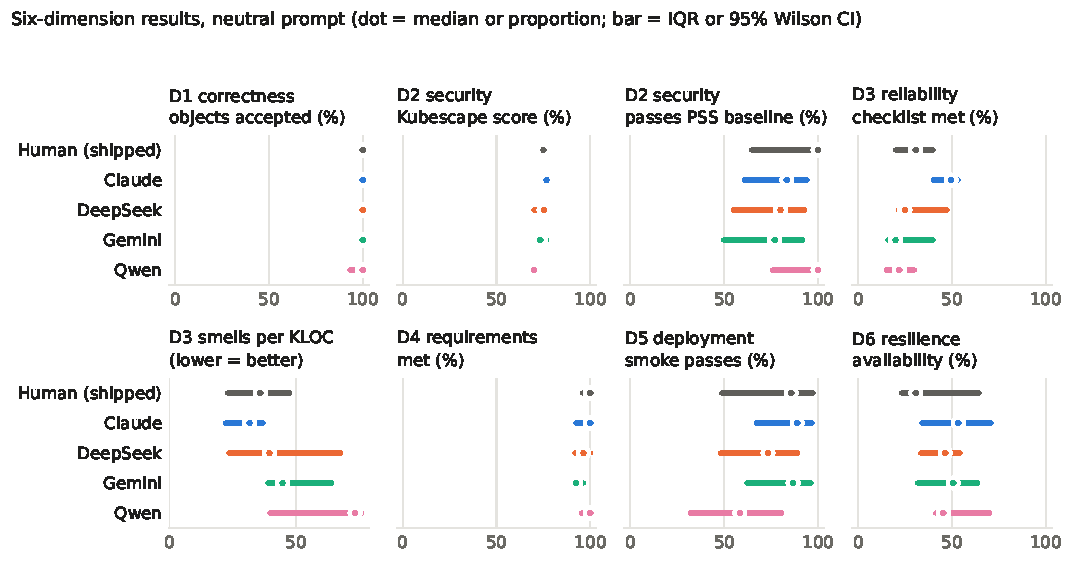
\includegraphics[width=\textwidth]{figures/fig_dimensions_neutral.pdf}
\caption{Six-dimension results for the neutral prompt, one row per source. Dots are medians (continuous metrics) or proportions (binary metrics); bars are interquartile ranges or 95\% Wilson intervals.}
\label{fig:dimensions-neutral}
\end{figure*}

\textbf{Correctness (D1).} Every human manifest and every neutral-prompt configuration from Claude, DeepSeek and GPT was accepted object by object by the API server. Gemini lost two of its 21 configurations, both for the Kubernetes Dashboard, because the provider withheld the response for reproducing training data too closely, and Qwen had all objects accepted in only 10 of its 15 configurations, mostly because it declared Services with several unnamed ports, which a schema validator accepts but the API server rejects. The share of objects accepted differs across sources (Kruskal-Wallis $H=21.81$, $p<0.001$) only because of Qwen (Dunn tests, Holm-adjusted, $p\le0.049$ against the human manifests, Claude, DeepSeek and GPT).

\textbf{Security (D2).} Under the neutral prompt, the generated configurations are about as secure, by static measures, as the manifests the projects ship. Median Kubescape compliance is 76.7\% for Claude, DeepSeek and Gemini, 79.8\% for GPT and 70.0\% for Qwen, against 75.0\% for the human manifests ($H=24.50$, $p<0.001$). GPT (Cliff's $\delta=+0.56$, large) and Claude ($\delta=+0.33$, small) lie above the human manifests and Qwen ($\delta=-0.64$, large) below them, but no pairwise difference with the human manifests survives the Holm adjustment; the significant pairs are Claude--Qwen and GPT--Qwen. Almost nothing reaches the \texttt{restricted} Pod Security Standard (0 of 7 human manifests; 0--24\% of each model's configurations), while 84--100\% of every source passes \texttt{baseline}. A hard-coded secret appears in 43\% of the human manifests and in 52--64\% of each model's configurations, a difference that is not significant ($\chi^2=1.08$, $p=0.956$).

\textbf{Static reliability (D3).} The generated configurations cover more of the reliability checklist than the shipped manifests: the median is 50.0\% for Claude and 54.0\% for GPT against 30.7\% for the human manifests ($\delta=+0.50$ and $+0.72$, both large), and the GPT--human difference is significant after adjustment ($p=0.040$). Gemini (40.0\%), DeepSeek (44.9\%) and Qwen (24.5\%) are close to the human level. KubeLinter smell density does not differ significantly between sources ($H=9.62$, $p=0.087$).

\textbf{Requirements (D4).} Requirement satisfaction is high for every source (medians 96--100\%) and does not differ significantly ($H=10.47$, $p=0.063$).

\textbf{Deployment (D5) and recovery (D6).} Every human manifest became fully Ready and six of the seven passed their smoke test; the exception, Sock Shop, became Ready but its front end no longer served the catalogue, because an image tag the manifest leaves unpinned has since moved. The models' neutral-prompt configurations became fully Ready in 60\% (Qwen) to 86\% (Claude) of cases and passed the smoke test in 47\% (Qwen) to 90\% (Claude). Neither rate differs significantly from the human manifests in any pairwise comparison (Fisher's exact test, all $p\ge0.60$), although seven human configurations give these tests little power. Time to Ready does not differ ($H=5.84$, $p=0.322$). Among configurations that reached fault injection, all recovered from all six injected faults except one GPT configuration; mean availability during the faults (median 30.8\% for the human manifests and 38--45\% per model) and mean recovery time (7.8~s and 13--17~s) do not differ significantly ($H=2.24$, $p=0.815$ and $H=1.77$, $p=0.880$). Restricting D6 to fully Ready configurations changes none of these results.
\textbf{Robustness.} Restricting the comparison to the five projects every model completed changes none of these conclusions: the Kubescape and checklist differences grow slightly (for GPT, $\delta=+0.76$ and $+0.93$; GPT--human checklist $p=0.010$) and the D1 difference remains confined to Qwen. Averaging the three samples of each project and pairing them with that project's human manifest ($n=7$ pairs per model) leaves only GPT's higher checklist coverage significant (median difference $+16.7$ points, Wilcoxon $p=0.031$); the other differences point the same way, but seven pairs give the test little power. Split by the intent of the human manifest, the two production-oriented manifests (Grafana and the Kubernetes Dashboard) score below most models on Kubescape compliance and checklist coverage, with large effect sizes that do not survive the adjustment for multiple comparisons with only two human configurations; the five demonstration-oriented projects reproduce the overall pattern.
The runtime comparisons are equally unchanged on the five common projects and at project level, where no D5 or D6 difference with the human manifests reaches significance.

\subsection{RQ2: Most frequent misconfigurations}\label{sec:res-rq2}

Table~\ref{tab:rahman} reports, for each source and prompt, the share of configurations exhibiting each of the eleven security misconfiguration categories of Rahman et al.\ \citep{rahman2023k8smisconfig}.

% generated by evaluation/tables.py -- do not edit
\begin{table*}[t]
\centering\small
\caption{Share of configurations (\%) exhibiting each security misconfiguration category of Rahman et al., detected with the rules of their SLI-KUBE tool. N = neutral prompt, P = production prompt.}\label{tab:rahman}
\begin{tabular}{lrrrrrrrrr}
\toprule
Category & Human & Claude N & Claude P & DeepSeek N & DeepSeek P & Gemini N & Gemini P & Qwen N & Qwen P \\ \midrule
Absent resource limit & 100 & 61 & 0 & 67 & 8 & 69 & 23 & 83 & 30 \\
Absent securityContext & 71 & 78 & 0 & 80 & 31 & 92 & 92 & 92 & 90 \\
Activation of hostIPC & 0 & 0 & 0 & 0 & 0 & 0 & 0 & 0 & 0 \\
Activation of hostNetwork & 0 & 0 & 0 & 0 & 0 & 0 & 0 & 0 & 0 \\
Activation of hostPID & 0 & 0 & 0 & 0 & 0 & 0 & 0 & 0 & 0 \\
Capability misuse & 0 & 0 & 0 & 0 & 0 & 0 & 0 & 0 & 0 \\
Docker socket mounting & 0 & 17 & 0 & 20 & 8 & 23 & 23 & 8 & 0 \\
Escalated privileges for child processes & 0 & 0 & 0 & 0 & 0 & 0 & 0 & 0 & 0 \\
Hard-coded secret & 57 & 67 & 60 & 60 & 62 & 69 & 69 & 75 & 80 \\
Insecure HTTP & 0 & 17 & 20 & 20 & 15 & 23 & 23 & 25 & 30 \\
Privileged securityContext & 0 & 0 & 0 & 0 & 0 & 0 & 0 & 0 & 0 \\
\bottomrule
\end{tabular}
\end{table*}


Three categories dominate for every source. A hard-coded secret appears in 57\% of the human manifests and in 64--71\% of each model's configurations under both prompts; an absent security context in 71\% of the human manifests and 76--86\% of neutral-prompt configurations; and an absent resource limit in every human manifest and in 24--79\% of neutral-prompt configurations. The production prompt removes most of the last two (for Claude, from 57\% and 76\% to 0\%; for GPT, from 24\% and 76\% to 5\% and 14\%) but leaves hard-coded secrets unchanged. Insecure HTTP is rare (0--25\%) and absent from the human manifests. Docker socket mounting (7--16\% of neutral configurations) occurs only for Sock Shop, whose bundled Compose file mounts the socket while its human manifest does not (Section~\ref{sec:disc-compose}). Host IPC, network and PID sharing, privileged containers, capability misuse and privilege escalation for child processes never occur. The scanners that detect these categories largely agree: on the five security checks Kubescape and Trivy both implement, Cohen's $\kappa$ is 0.88 overall (0.70--1.00 per check).

Compared with the ChatGPT configurations of 2023 studied by Zhang et al.\ \citep{zhang2024genaismells}, current models produce far fewer of the six KubeLinter smells per thousand lines under the neutral prompt: 7.4--10.7 instances of a writable root filesystem against 22.7, 10.8--16.1 of a container that may run as root against 22.8, 1.8--12.4 of unset CPU or memory requests against 45.5 each, and almost no dangling Services (0--0.2 against 6.7). These densities are close to those of the human manifests (5.9--7.7 for the first four smells), with Qwen the highest of the five models. Because our unit is a whole multi-object configuration and Zhang et al.'s a manifest file, the comparison uses density; the share of configurations with at least one instance is inflated by the larger unit and is not compared.

\subsection{RQ3: Differences between models and consistency}\label{sec:res-rq3}

Under the neutral prompt the models differ significantly in Kubescape compliance ($H=23.39$), checklist coverage ($H=18.94$), Polaris score ($H=19.38$) and the share of objects accepted ($H=19.92$; all $p<0.001$). The differences come almost entirely from Qwen, which scores below Claude and GPT on every one of these metrics, and from GPT's higher checklist coverage than Gemini's. Under the production prompt the models separate much more clearly ($H=60.80$ for Kubescape compliance, $46.91$ for checklist coverage and $49.19$ for Polaris score, all $p<0.001$): Claude and GPT form a top group, DeepSeek a middle one, and Gemini and Qwen a bottom one, with every pairwise difference between the top and bottom groups significant after adjustment. Repeating the analysis on the five projects every model completed reproduces both orderings. Requirement satisfaction does not differ between models under either prompt.

The three samples drawn for each model, project and prompt are most alike for Gemini (median across-sample standard deviation 0 for Kubescape compliance and checklist coverage) and least alike for Qwen (15.8 points for the share of objects accepted and 11.1 for checklist coverage); Claude, DeepSeek and GPT lie in between.
The runtime outcome is much less repeatable than the static scores. All three samples of a cell agree on whether the configuration becomes fully Ready in 86\% of cells for Claude, 71\% for Gemini, 50\% for GPT and Qwen and 43\% for DeepSeek, and agree on the smoke-test outcome in 64--71\% of cells for every model. Between models, deployment success differs little under the neutral prompt, where only the smoke-test rate differs ($\chi^2=10.78$, $p=0.029$; Qwen 47\% against 76--90\% for the others), but clearly under the production prompt (Ready $\chi^2=12.25$, $p=0.016$; smoke test $\chi^2=13.95$, $p=0.007$), where Gemini's configurations pass the smoke test in 90\% of cases and DeepSeek's in 38\%.

\subsection{RQ4: Runtime behaviour and the predictive value of static analysis}\label{sec:res-rq4}

Table~\ref{tab:d5-failures} classifies why LLM-generated configurations failed to become fully Ready. Each class is assigned from the cluster's own record of the failed deployment (container exit codes and reasons, restart counts and warning events), captured before the deployment is torn down.

% generated by evaluation/tables.py -- do not edit
\begin{table}[t]
\centering\small
\caption{Classified reason for LLM-generated configurations that did not become fully Ready (D5), by prompt.}\label{tab:d5-failures}
\begin{tabular}{lrrr}
\toprule
Failure class & Neutral & Production & Total \\ \midrule
CrashLoopBackOff & 9 & 14 & 23 \\
NotReady(probe) & 3 & 7 & 10 \\
ContainerCreating & 1 & 1 & 2 \\
no workloads & 1 & 0 & 1 \\
\bottomrule
\end{tabular}
\end{table}


Of the 198 generated configurations, 180 had every object accepted and were deployed, 128 became fully Ready, 136 passed their smoke test and 118 did both. The two outcomes disagree in 28 configurations. In 18, the application served every smoke-test request while some workload never became Ready (six from Gemini, four each from DeepSeek and Qwen, three from GPT and one from Claude), most often an auxiliary component carried over from the Compose file, such as Sock Shop's load generator. In the other 10, every workload was Ready but the application did not work: in six a Service, RBAC object or NetworkPolicy needed on the request path was rejected or misdirected, in one a placeholder domain was enforced, and in three the cause could not be determined, because diagnostics are captured only for configurations that do not become Ready. Table~\ref{tab:root-causes} assigns a root cause to each of the 81 configurations (80 generated and one human) that were not both fully Ready and passing their smoke test; 51 of the mechanisms are directly visible in the cluster's record, 20 are inferred from the manifest together with the observed status, 6 are supported by a matched contrast and 4 remain undetermined. The most frequent are host-level Compose services that fail while the application works (10), invalid YAML or objects the API server rejects (8), hardening that stops a database (7) and liveness probes that kill slow-starting services (6).

% generated by evaluation/tables.py -- do not edit
\begin{table*}[t]
\centering\small
\caption{Root cause of every configuration that was not both fully Ready and passing its smoke test, by model and prompt (N = neutral, P = production). Obs.\ = cases whose mechanism is directly visible in the cluster's record (exit reason, log lines, events, rejected objects or provider stop reason); the remainder are inferred from the manifest together with the observed status, or, for two mechanisms, supported by a matched contrast.}\label{tab:root-causes}
\begin{tabular}{lrrrrrrrrr}
\toprule
Mechanism & Claude & DeepSeek & Gemini & GPT & Qwen & N & P & Human & Obs. \\ \midrule
\multicolumn{10}{l}{\textit{Hardening blocks the workload}} \\
\quad Capability drop or fixed UID stops the database & 3 & 2 & 0 & 2 & 0 & 0 & 7 & 0 & 3/7 \\
\quad runAsNonRoot on an image whose user cannot be verified & 0 & 1 & 0 & 2 & 0 & 1 & 2 & 0 & 0/3 \\
\quad Service-account token disabled for a component that needs the API & 0 & 0 & 0 & 1 & 0 & 0 & 1 & 0 & 1/1 \\
\quad NetworkPolicy blocks a documented internal route & 1 & 0 & 0 & 1 & 0 & 1 & 1 & 0 & 0/2 \\
\multicolumn{10}{l}{\textit{Probes and resource limits}} \\
\quad Liveness/startup probe kills a slow-starting service & 5 & 0 & 0 & 1 & 0 & 2 & 4 & 0 & 2/6 \\
\quad Memory limit too low (OOMKilled) & 0 & 1 & 0 & 1 & 0 & 1 & 1 & 0 & 2/2 \\
\quad Probe on the wrong port or path & 0 & 3 & 0 & 0 & 0 & 0 & 3 & 0 & 1/3 \\
\quad Probe calls a binary the image does not ship & 0 & 0 & 1 & 0 & 0 & 1 & 0 & 0 & 0/1 \\
\quad HTTP probe on a component without a server & 0 & 0 & 0 & 0 & 4 & 1 & 3 & 0 & 0/4 \\
\multicolumn{10}{l}{\textit{Compose file translated literally}} \\
\quad Host-level Compose services break the application & 0 & 1 & 0 & 0 & 0 & 1 & 0 & 0 & 0/1 \\
\quad Host-level Compose services fail; application works & 1 & 2 & 6 & 1 & 0 & 7 & 3 & 0 & 10/10 \\
\multicolumn{10}{l}{\textit{Wrong values or references}} \\
\quad Service targets the wrong container port & 0 & 0 & 0 & 0 & 1 & 1 & 0 & 0 & 1/1 \\
\quad API server address overridden & 0 & 1 & 0 & 0 & 0 & 0 & 1 & 0 & 0/1 \\
\quad Volume references an undefined Secret & 0 & 1 & 0 & 0 & 0 & 1 & 0 & 0 & 1/1 \\
\quad RBAC does not allow updating the CSRF Secret & 0 & 0 & 0 & 1 & 3 & 2 & 2 & 0 & 0/4 \\
\quad No writable /tmp volume on a distroless image & 0 & 0 & 0 & 0 & 1 & 1 & 0 & 0 & 1/1 \\
\quad Image from a non-existent repository & 0 & 0 & 0 & 0 & 2 & 0 & 2 & 0 & 2/2 \\
\quad Required variable set to an empty value & 0 & 2 & 0 & 1 & 0 & 1 & 2 & 0 & 3/3 \\
\quad Non-existent command-line flag & 0 & 0 & 0 & 3 & 0 & 1 & 2 & 0 & 3/3 \\
\quad Placeholder domain enforced & 0 & 0 & 0 & 1 & 0 & 0 & 1 & 0 & 1/1 \\
\quad Points at a database host that does not exist & 0 & 1 & 0 & 1 & 0 & 1 & 1 & 0 & 2/2 \\
\quad TLS required by the client, not offered by the database & 0 & 1 & 0 & 0 & 0 & 0 & 1 & 0 & 1/1 \\
\multicolumn{10}{l}{\textit{Invalid or missing output}} \\
\quad Invalid YAML or object rejected by the API server & 0 & 1 & 0 & 0 & 7 & 4 & 4 & 0 & 8/8 \\
\quad RBAC object rejected (unquoted resource name) & 0 & 2 & 0 & 0 & 0 & 0 & 2 & 0 & 2/2 \\
\quad Reply ends before the YAML block closes & 0 & 0 & 1 & 0 & 2 & 1 & 2 & 0 & 3/3 \\
\quad Provider withheld the reply (recitation) & 0 & 0 & 3 & 0 & 0 & 2 & 1 & 0 & 3/3 \\
\multicolumn{10}{l}{\textit{Other}} \\
\quad Cause not determined & 0 & 3 & 0 & 1 & 0 & 2 & 2 & 0 & 0/4 \\
\quad Unpinned image tag drifted & 0 & 0 & 0 & 0 & 0 & 0 & 0 & 1 & 1/1 \\
\midrule
Total & 10 & 22 & 11 & 17 & 20 & 32 & 48 & 1 & 51/81 \\
\bottomrule
\end{tabular}
\end{table*}


Static scores are a poor guide to runtime behaviour (all correlations Holm-adjusted, pooled over both prompts). No static security or reliability score is associated with becoming fully Ready; only requirement satisfaction is, weakly ($r_{pb}=+0.21$, $p=0.047$). For the smoke test the associations run the wrong way: configurations with higher Polaris scores ($r_{pb}=-0.29$, $p<0.001$) and higher Kubescape compliance ($-0.23$, $p=0.026$) pass it less often, and those with more KubeLinter smells pass it more often ($+0.28$, $p=0.001$). The only positive association with a runtime measure is between checklist coverage and availability during faults ($\rho=+0.30$, $p=0.003$), which is expected because the checklist rewards replicas and disruption budgets. Because the production prompt raises the static scores and lowers deployment success at the same time (Section~\ref{sec:res-rq5}), part of the negative association reflects the prompt rather than a within-prompt relationship; either way, a higher static score does not indicate a configuration more likely to work.

\subsection{RQ5: Effect of requesting production-ready output}\label{sec:res-rq5}

Figure~\ref{fig:prompt-effect} shows, for each model, how the production prompt moves each headline metric relative to the neutral prompt; Table~\ref{tab:overview-production} gives the production-prompt values.

\begin{figure*}[t]
\centering
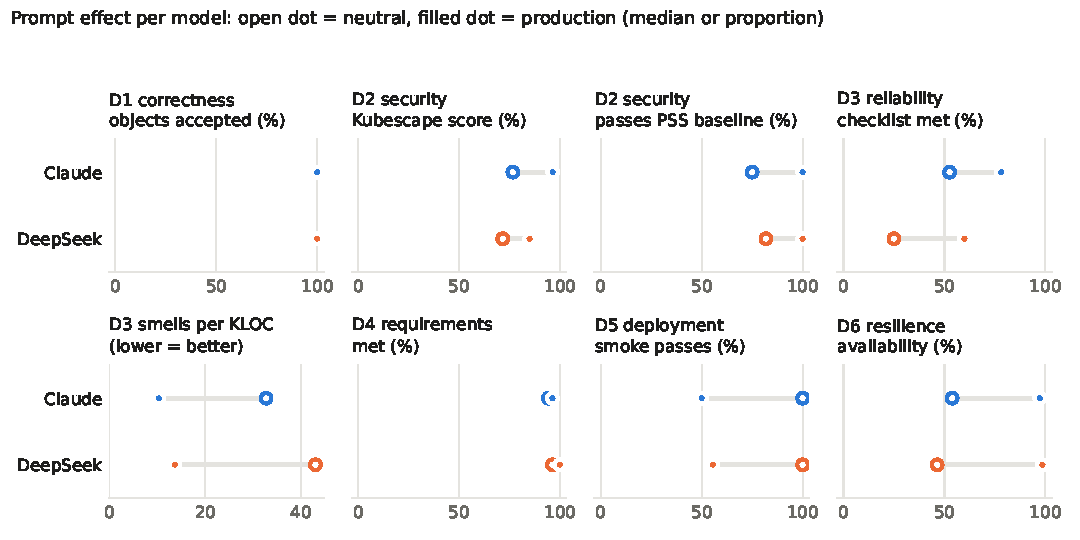
\includegraphics[width=\textwidth]{figures/fig_prompt_effect.pdf}
\caption{Effect of the production prompt per model: open dot = neutral prompt, filled dot = production prompt (median or proportion).}
\label{fig:prompt-effect}
\end{figure*}

% generated by evaluation/tables.py -- do not edit
\begin{table*}[t]
\centering\small
\caption{Six-dimension results, production prompt. Binary rows: percentage (count/n); continuous rows: median [interquartile range]. The human column is the shipped manifest of each project (one per project). D5 time to Ready and D6 are conditional on deployment.}\label{tab:overview-production}
\begin{tabular}{lrrr}
\toprule
Metric & Human & Claude & DeepSeek \\ \midrule
Configurations & 7 & 6 & 11 \\ \midrule
D1 all objects API-accepted & 100 (7/7) & 100 (6/6) & 73 (8/11) \\
D2 passes PSS baseline & 100 (7/7) & 100 (6/6) & 90 (9/10) \\
D2 passes PSS restricted & 0 (0/7) & 17 (1/6) & 20 (2/10) \\
D2 hard-coded secret & 43 (3/7) & 100 (6/6) & 70 (7/10) \\
D5 fully Ready & 100 (7/7) & 33 (2/6) & 36 (4/11) \\
D5 smoke test passes & 86 (6/7) & 33 (2/6) & 36 (4/11) \\
D6 recovers from all 6 faults & 100 (7/7) & 100 (2/2) & 100 (4/4) \\
\midrule
D2 Kubescape compliance (\%) & 75.0 [73.0, 76.6] & 95.9 [92.3, 96.4] & 83.3 [80.0, 86.2] \\
D3 reliability checklist (\%) & 30.7 [20.0, 40.0] & 70.4 [61.3, 79.4] & 59.4 [57.3, 67.7] \\
D3 smells per KLOC & 36.0 [23.1, 47.5] & 10.6 [10.3, 17.6] & 13.7 [7.8, 17.1] \\
D4 requirements met (\%) & 100.0 [95.8, 100.0] & 98.2 [96.3, 100.0] & 98.2 [96.3, 100.0] \\
D5 time to Ready (s) & 20.1 [14.6, 64.0] & 56.4 [55.1, 57.7] & 22.1 [16.2, 27.9] \\
D6 availability under faults (\%) & 30.8 [23.2, 64.6] & 20.4 [20.4, 20.5] & 98.5 [80.1, 99.2] \\
\bottomrule
\end{tabular}
\end{table*}


Asking for production-ready output improves every static measure, for every model. Paired by model, project and sample, median Kubescape compliance rises by 10.0 points ($p<0.001$; significant for each model, from $+3.3$ for Gemini to $+19.8$ for Claude), high and critical Trivy findings fall by 1.5 (by 10 for Claude and 8 for GPT; not significant for Gemini or Qwen), checklist coverage rises by 22.5 points and Polaris score by 13.0 (both significant for every model), and KubeLinter smell density falls by 16.3 per thousand lines (not significant for Gemini). The share of configurations passing the \texttt{restricted} Pod Security Standard rises sharply: 27 configurations pass only under the production prompt and one only under the neutral one (exact McNemar $p<0.001$), led by Claude (11 to 0), DeepSeek and GPT (7 to 0 each). Requirement satisfaction does not change.
Deployment, in contrast, becomes less likely to succeed. Of the configuration pairs whose outcome differs between the prompts, 21 became fully Ready only under the neutral prompt and 5 only under the production prompt (exact McNemar $p=0.002$); for the smoke test the counts are 23 and 7 ($p=0.005$). The loss is spread across Claude, DeepSeek, GPT and Qwen, but is individually significant only for DeepSeek's smoke test (9 against 1, $p=0.021$); Gemini is the exception, with 1 and 2 pairs in each direction. The configurations that do deploy under both prompts are more resilient to faults under the production prompt: median availability during fault injection rises by 9.8 points ($p<0.001$; for Claude by 28.3, $p=0.003$), while recovery time does not change ($p=0.371$) and every configuration that recovered under one prompt also recovered under the other.

\section{Discussion}\label{sec:discussion}

% Counts are taken from evaluation/d5_root_causes.csv, evaluation/analysis/report.md and robust_report.md.

\subsection{Hardening that breaks the workload it hardens}\label{sec:disc-hardening}

Under the production prompt, a recurring cause of failure is a security control applied without regard to the image it constrains. Eight configurations (three each from Claude and DeepSeek and two from GPT, all under the production prompt) hardened their database so that it could not start. In seven, the database container (PostgreSQL in six, MySQL in one) keeps its root-based entrypoint but has every Linux capability dropped: the entrypoint must take ownership of its data directory and then switch to an unprivileged user, and without the corresponding capabilities it can do neither. In the eighth, the database runs as a fixed non-root user with its data directory at the root of a volume it does not own, so initialisation cannot set the directory's permissions. These eight configurations score as well on Kubescape as the other production-prompt configurations (median compliance 89.6\% in both groups), so the scanner gives no sign of the defect.

Two further mechanisms follow the same pattern, each a recognised practice in isolation. Liveness or startup probes whose time budget is shorter than a slow-starting Java service needs kill each container before it finishes starting, so the services restart indefinitely; this accounts for six failures (five from Claude, four under the production prompt), observed directly in two (kubelet kills with no out-of-memory reason, and log lines showing the services still initialising) and inferred for the other four from the same probe settings and readiness record. A least-privilege NetworkPolicy that admits traffic to the Kubernetes Dashboard's metrics scraper only from the dashboard's own pods blocks the dashboard's default route to the scraper, which passes through the API server's service proxy; samples from the same model with an identical policy but a direct scraper address connected normally. This accounts for two failures, one supported by that matched contrast and the other inferred from the same policy, rather than by a controlled experiment. The third NetworkPolicy failure in Table~\ref{tab:root-causes} is a different mechanism: an Online Boutique policy admits internal traffic only from pods carrying a label that no pod carries.

The production prompt therefore buys static compliance partly at the cost of deployability (Section~\ref{sec:res-rq5}); static gains matter only for configurations that still deploy.

\subsection{Translating the Compose file too literally}\label{sec:disc-compose}

Every model receives the project's Docker Compose file, and models tend to translate it service by service. Where the Compose file reflects a Docker-host setup that the maintainers deliberately left out of their Kubernetes manifests, this faithfulness is a defect. Sock Shop's Compose file mounts the host's Docker socket into one service and runs a one-shot load generator; its Kubernetes manifest contains neither. Under the neutral prompt, 12 of the 15 Sock Shop configurations mount the socket (all three samples from Claude, DeepSeek and Gemini), against 4 of 15 under the production prompt, and 27 of the 30 include the load generator. Access to the Docker socket is equivalent to root on the node \citep{rahman2023k8smisconfig}, and the socket does not exist on nodes whose container runtime is not Docker Engine, as on the evaluation cluster. A load generator run as a long-lived Deployment restarts indefinitely, and in several samples its command invokes a start-up script that does not exist in the image. The load generator is the most frequent single cause of a configuration that serves correctly but is not fully Ready (Table~\ref{tab:root-causes}).

\subsection{What static analysis misses}\label{sec:disc-static}

Several failures were not visible to the static scanners. A memory limit too tight for a Java service is recorded by the cluster as an out-of-memory kill, but no scanner relates a limit to the workload it constrains. A database that cannot start under its security context passes every structural check, and so does a probe aimed at a path the image does not serve. Other defects are caught before deployment but are easy to miss in review: in two DeepSeek configurations, an unquoted RBAC resource name containing colons was parsed by YAML as a mapping, the API server rejected the whole Role, and the dashboard started without its permissions. Consistent with these cases, higher static security and reliability scores show no positive association with deployment success (Section~\ref{sec:res-rq4}); only requirement satisfaction, which checks that the documented components and settings are present, is weakly associated with it. Each of these defects surfaced only at deployment.

\subsection{``Ready'' is not the same as ``working''}\label{sec:disc-ready}

Kubernetes considers a workload Ready when its readiness probe passes, or immediately when it has none. The human Sock Shop manifest defines no readiness probes, so its slow Java services are reported Ready long before they accept connections, while several generated configurations serve every request correctly with an auxiliary workload not Ready. In this study the two outcomes disagree for 28 of the 198 generated configurations (18 serve correctly without being fully Ready and 10 are fully Ready without serving correctly). Reporting both readiness and a smoke test avoids rewarding missing probes and penalising non-essential components.

\subsection{Memorisation}\label{sec:disc-memorisation}

Two observations bear on the contamination threat (Section~\ref{sec:threats}). First, Gemini's provider withheld three responses for the Kubernetes Dashboard (two under the neutral prompt, one under the production prompt) because they reproduced training data too closely; the project's official manifest is widely published. Second, some models' configurations are more similar to the published human manifest than to the other models' configurations for the same project, which is the pattern expected if a published manifest is being reproduced. The excess is clearly positive for Claude on the Kubernetes Dashboard (Jaccard $+0.35$) and Emojivoto ($+0.23$) and for Gemini on Sock Shop ($+0.23$), and close to zero or negative elsewhere. For Claude, access to the human manifests during generation is ruled out by the session transcripts (Section~\ref{sec:method-generation}), so this similarity reflects what the model learned in training. Neither observation affects the scoring, but both limit how far results on widely published projects can be read as reasoning from documentation.

\subsection{Generalisation beyond the evaluated projects}\label{sec:disc-generalisation}

The failure mechanisms identified above arise from how generated configurations interact with common images and Kubernetes defaults rather than from any single application: database images with root-based entrypoints, slow-starting JVM services and Compose files written for a Docker host are widespread. We therefore expect these mechanisms to recur in similar projects. This expectation remains to be tested, and the per-project rates reported here should not be extrapolated to applications of other kinds.

\subsection{Implications}\label{sec:disc-implications}

For practitioners, the results suggest three checks before adopting a generated configuration: deploy it and exercise it, rather than relying on how it reads or scores; review every hardening setting against the documented behaviour of the image it constrains, in particular capability drops and fixed user IDs on database images and liveness probes on slow-starting services; and treat host-level settings carried over from a Compose file (socket mounts, host paths, one-shot services) as suspect. Asking a model for ``production-ready'' output makes these checks more necessary, not less. For tool builders, the results suggest scanner rules that relate a security setting to the image it is applied to. For researchers, benchmarks of generated infrastructure code should include execution, since a scanner score did not indicate which configurations would work.

\section{Threats to Validity}\label{sec:threats}

\textbf{Model access.} The models were reached through different routes (Table~\ref{tab:models}), a known risk for studies that use LLMs \citep{sallou2024breaking}. Three were generated through conversational interfaces rather than a raw API: Claude through Claude Code subagents, which add their harness's system prompt to ours, and GPT and DeepSeek through their web chats, whose own system prompts and defaults are outside the study's control. Temperature and the output limit were therefore controlled only for Gemini and Qwen, which affects the consistency comparison of RQ3 more than any other result. GPT was generated with ChatGPT's default model, so its exact version is not known; it answered with a medium reasoning effort that was left unchanged. Its web sessions were operated by a third party following a written protocol (a new temporary, unpersonalised chat per prompt, no tools, no follow-up, replies copied unedited) whose adherence could not be observed directly, and for 16 of its 42 prompts, from the three projects with the longest documentation, the interface turned the pasted prompt into an attached file with identical content. Gemini is a flash-tier model rather than the planned Pro tier, and its hidden reasoning tokens count against its 8,192-token output limit. Qwen's free tier rejects the two largest projects' prompts, so its missing cells reflect access, not quality. A sixth model, Llama, was dropped before the main run because no working access route was found.

\textbf{Training-data contamination.} All projects are public, and only two of the seven manifest repositories have fewer than 2,000 GitHub stars, so a model may reproduce a memorised manifest rather than reason from the documentation. Provider refusals for recitation are recorded, and each model's similarity to the human manifest is compared with its similarity to the other models' configurations for the same project, so that only an excess over the peer level is read as reproduction (Section~\ref{sec:disc-memorisation}). Reproduction would pull a model's configurations toward the human manifest and so shrink the differences reported for RQ1.

\textbf{Selection of projects and of the human baseline.} Results describe these seven projects, not application classes in general (Section~\ref{sec:disc-generalisation}). The set was fixed after a two-project pilot and before the main run. Because a project was selected only if its human manifest deployed on the evaluation cluster, the human D5 outcomes are partly true by construction, and the selection favours applications that run on a local cluster; human runtime results are therefore reported as a reference only.

\textbf{Evaluation cluster.} D5 and D6 are measured on a four-node \texttt{kind} cluster on a single host. Cloud load balancers, multi-zone scheduling and production storage are not exercised, and absolute times should not be read as representative of production. \texttt{kind}'s local-path storage does not apply a pod's \texttt{fsGroup}, which could make a database fail here that would start elsewhere. None of the eight database failures depends on it: seven run the container as root with every capability dropped, which prevents the entrypoint from changing file ownership or switching user whatever the volume's group, and the eighth fails because its data directory is owned by another user, which \texttt{fsGroup} does not change.

\textbf{Measurement adjustments.} The pipeline was corrected 25 times during the study (Appendix~\ref{app:fixes}); each correction was logged with its trigger, applied to every configuration it could affect and followed by re-evaluation. All were made after generation had begun, and because most were found while diagnosing failures, they are one-sided: 8 affected only the running of the pipeline, 3 made scoring stricter, and 14 removed a failure that the investigation traced to the measurement or to an undocumented prerequisite, never a success that turned out to be spurious. The deployment results are robust to leaving out any one project (Section~\ref{sec:res-rq5}). Two adjustments supply facts the bundles lack (image aliases and start-up prerequisites, Section~\ref{sec:method-pipeline}); they apply to 29 generated configurations and to no human manifest. In the worst case, in which every adjusted configuration that succeeded would otherwise have failed, the share of generated configurations both fully Ready and passing the smoke test falls from 59.6\% to 51.0\%. Four of the dashboard failures concern a start-up Secret that the documentation never mentions: once the Secret is supplied, these configurations fail because their RBAC rules do not let the dashboard update it, which a deployer would also have to discover. Three configurations set a required variable to an empty string, which the application rejects; the start-up adjustment fires only when a variable is absent, so they are scored as failing.

\textbf{Labelling and tools.} Root-cause labels were assigned by a single rater, drafted with the help of an AI assistant from the same model family as one of the evaluated models (Claude). The blind second labelling pass was also made by a Claude model, not by a second human: it shows that the labels follow from the recorded evidence ($\kappa=0.84$), but it cannot rule out errors that models of one family share. The evidence level of each label is reported, and every label is published with its evidence so that it can be re-rated. The static tools are imperfect and disagree with one another, so their findings are read as what these pinned tool versions detect; agreement between the two security scanners is reported. Redaction decisions followed a written rule set, with every redaction logged and reviewed by a second author, but borderline cases remain possible. Facts that the bundles do not contain are excluded from D4, while the default ports of widely used database images are treated as general knowledge and scored.

\textbf{Resilience measurement.} The two injected faults are handled by Kubernetes controllers whatever the configuration says, so recovery success barely discriminates, and downtime depends mainly on replica count. D6 therefore characterises the replica choices a model makes rather than a broader notion of resilience; faults such as node drains or resource pressure would test more of a configuration's choices.

\textbf{Drift.} Providers update the weights behind a model identifier without notice, and an unpinned image tag resolves to whatever is current. Generation dates are recorded for every configuration, and images were resolved in November 2026. Tag drift affects the human baselines too: the human Sock Shop manifest references \texttt{mongo} without a tag, which now resolves to a release whose wire protocol the project's 2017 cart service no longer speaks; re-deploying with the image pinned to an older release passed, but the baseline is scored as published.

\section{Conclusion}\label{sec:conclusion}

This study compared Kubernetes configurations generated by five current LLMs with the manifests shipped by the same seven open-source projects, deploying and exercising every configuration rather than only scanning it. Each model received only the project's own documentation, under a neutral and a production-oriented prompt, three times each.

First, generated configurations are largely valid: 92.9\% are schema-valid, and requirement satisfaction is high for every model. Under a neutral prompt their static security is close to what these projects ship (within about ten Kubescape points per model), and GPT's and Claude's cover more of the reliability checklist. Validity does not imply a working deployment, however: only 59.6\% of the generated configurations became fully Ready and passed their smoke test, and higher static security and reliability scores showed no positive association with success. Second, asking for production-ready output raises static scores while lowering deployment success: across model--project cells, median Kubescape compliance rose by 9 points and checklist coverage by 22.5, while the smoke-test pass rate fell from 76.8\% to 60.6\%. The added failures come from hardening applied without regard to the image (capability drops that stop databases from starting, liveness probes that kill slow-starting services). Third, models translate a project's Docker Compose file too literally, carrying over host-level settings such as a mounted Docker socket that the maintainers deliberately left out of their Kubernetes manifests.

A generated configuration should therefore be deployed and exercised before it is trusted, and its hardening settings checked against the images they constrain. Future work should extend the evaluation to more projects, to managed multi-node clusters and to faults that exercise configuration choices (node drains that test disruption budgets, resource pressure, dependency restarts), and should test whether the cluster's record of a failed deployment, which identified a cause for nearly every failure here, lets a model repair its own configuration.


\FloatBarrier
\bibliographystyle{cas-model2-names}
\bibliography{references}

\end{document}
